\lstset{language=bash}
\chapter{OpenXENManager}
\section{Présentation}
XenseMaking Project développe un client lourd, ainsi qu'un client
web, pour manager XenServer. C'est un clone du XenCenter, qui fonctionne
avec Linux, BSD, Windows et MacOSX, alors que le XenCenter ne fonctionne
qu'avec Windows. OpenXenManager/OpenXenCenter un le client lourd qui
permet de manager XenServer.Il a été développé en Python avec pygtk
et gtk-vnc.
Les fonctionnalités actuellement implémentées sont les suivantes :
\begin{itemize}
\item monitoring des machines virtuelles - accès à la console des machines virtuelles
\item opérations d'administration (démarrage, arrèt, reboot, ...)
\item création de machines virtuelles
\end{itemize}
\section{Installation}
Pour l'installation nous avons besoin des paquets suivants:
\begin{lstlisting}
apt-get install subversion bzip2 python-glade2 python-gtk-vnc shared-mime-info graphviz
\end{lstlisting}
On télécharge la dernière version d'openxenmanager dans le dépot subversion
\begin{lstlisting}
svn co https://openxenmanager.svn.sourceforge.net/svnroot/openxenmanager openxenmanager
\end{lstlisting}
On se déplace dans le répertoire trunk:
\begin{lstlisting}
cd openxenmanager/trunk
\end{lstlisting}
Finalement on lance openxenmanager avec la commande suivante:
\begin{lstlisting}
python window.py
\end{lstlisting}
Une interface graphique d'openxenmanger apparaît.

\section{Problèmes rencontrés avec OpenXenManager}

A l'origine, OpenXenManager est destiné à manager XenServer qui fonctionne uniquement avec le système d'exploitation windows.\\Malheureusement nous travaillons dans un environement différent de windows, notre premier problème fût de trouver un équivalent sous linux.
Après plusieurs jours de recherche, nous avons trouvé un programme susceptible de fonctionner avec OpenXenManager qui s'appelle Xen cloud Platform.
Très peu de documentation sont disponibls sur internet, nous avons suivi un tutoriel qui nous semble être l'un des mieux explicatif pour essayer de l'installer mais celui ci n'a pas fonctionné.
Nous allons vous présenter un extrait des étapes de la configuration ansi que les problèmes rencontrés.
\subsection{Préparation du système}
La première étape consistait à préparer le système pour l'installation:
\begin{itemize}
\item Rajouter des dépôts dans le source.list
\item Récupérer la clé pour y accéder.
\end{itemize}

\subsubsection{Problème rencontrés durant cette étape}

Après avoir rajouter les dépôts dans le /etc/apt/source.listes:

\begin{lstlisting}
deb http://ppa.launchpad.net/ubuntu-xen-org/xcp-unstable/ubuntu oneiric main 
deb-src http://ppa.launchpad.net/ubuntu-xen-org/xcp-unstable/ubuntu oneiric main
\end{lstlisting}
Et utilisé la commande suivante:
\begin{lstlisting}
apt-key adv --keyserver keyserver.ubuntu.com --recv-keys 9273A937
\end{lstlisting}

On obtient le message suivant :

\begin{lstlisting}
 root@griffon-61:~# apt-key adv --keyserver keyserver.ubuntu.com --recv-keys 9273A937
 Executing: gpg --ignore-time-conflict --no-options --no-default-keyring --secret-keyring /tmp/tmp.BoYHj5Rkxz --trustdb-name /etc/apt/trustdb.gpg --keyring /etc/apt/trusted.gpg --primary-keyring /etc/apt/trusted.gpg --keyserver keyserver.ubuntu.com --recv-keys 9273A937
 gpg: requesting key 9273A937 from hkp server keyserver.ubuntu.com
 gpg: keyserver timed out
 gpg: keyserver receive failed: keyserver error
\end{lstlisting}

Il semblerait que nous ne pouvions pas accéder au serveur pour récupérer la clé.

Ensuite nous devions installer python-software-properties une dépendance requise pour que XCP fonctionne.
En faisant un
\begin{lstlisting} 
apt-get update
\end{lstlisting}
avant d'installer python-software-properties on obtient le message suivant:

\begin{lstlisting}
W: GPG error: http://ppa.launchpad.net oneiric Release: The following signatures couldn't be verified because the public key is not available: NO_PUBKEY 79B578FB9273A937
\end{lstlisting}

Comme nous n'avons pas récupéré la clé, il nous est impossible d'installer la dépendance.

\subsection{Installation de XCP}

Il faut tout d'abord ajouter les dépôts d'XCP avec la commande suivante:
\begin{lstlisting}
add-apt-repository ppa:ubuntu-xen-org/xcp-unstable
\end{lstlisting}

\subsubsection{Prblèmes rencontrés durant cette étape}
Il s'en suit un échec de la commande.
\begin{lstlisting}  
root@griffon-61:~# add-apt-repository ppa:ubuntu-xen-org/xcp-unstable
Traceback (most recent call last):
File "/usr/bin/add-apt-repository", line 88, in <module>
ppa_info = get_ppa_info_from_lp(user, ppa_name)
File "/usr/lib/python2.7/dist-packages/softwareproperties/ppa.py", line 80, in get_ppa_info_from_lp
curl.perform()
pycurl.error: (28, 'connect() timed out!')
\end{lstlisting}
Il nous est impossible d'ajouter les dépôts pour récupérer XCP.
Pour les étapes suivantes, nous n'avons rencontré aucun problème:
\begin{itemize}
\item Installation de dépendances pour XCP
\item Installation de XCP
\end{itemize}
\begin{lstlisting}
apt-get update
apt-get install openvswitch-datapath-dkms
\end{lstlisting}
Tout s'installe correctement, ce n'est que lors de l'installation de Xen Cloud Platform que plusieurs problèmes sont survenus.
\begin{lstlisting}
apt-get update
apt-get install xcp-xapi
apt-get install xcp-xe
\end{lstlisting}


\begin{lstlisting}
Starting the XCP networking daemon: .............................. * failed to start xcp-networkd.

invoke-rc.d: initscript xcp-networkd, action "start" failed.
dpkg: error processing xcp-networkd (--configure):
subprocess installed post-installation script returned error exit status 1
dpkg: dependency problems prevent configuration of xcp-xapi:
xcp-xapi depends on xcp-networkd; however:
Package xcp-networkd is not configured yet.
dpkg: error processing xcp-xapi (--configure):
dependency problems - leaving unconfigured
dpkg: dependency problems prevent configuration of xcp-guest-templates:
xcp-guest-templates depends on xcp-xapi; however:
Package xcp-xapi is not configured yet.
dpkg: error processing xcp-guest-templates (--configure):
dependency problems - leaving unconfigured
Setting up xcp-vncterm (0.1.1-1ubuntu1) ...
Processing triggers for libc-bin ...
ldconfig deferred processing now taking place
No apport report written because the error message indicates its a followup error from a previous failure.
No apport report written because the error message indicates its a followup error from a previous failure.
Processing triggers for initramfs-tools ...
update-initramfs: Generating /boot/initrd.img-3.0.0-12-server
Errors were encountered while processing:
xcp-networkd
xcp-xapi
xcp-guest-templates
E: Sub-process /usr/bin/dpkg returned an error code (1)
\end{lstlisting}

Suite aux nombreux problèmes rencontrés sur ce sujet nous avons décidé de passer sur notre second projet virt-manager.

\section{Xen Cloud Platform}
Le fait de passer au second sujet nous a permis de débloquer la situation avec OpenXenManager.
En effe, nous avons pu installer XCP grâce à virt-manager dans une machine virtuelle avec l'aide d'une image iso d'XCP téléchargée depuis le site officiel.
L'installation est simple, depuis la machine virtuelle on boot sur l'image iso et l'on suit les étapes suivantes.
\begin{center}
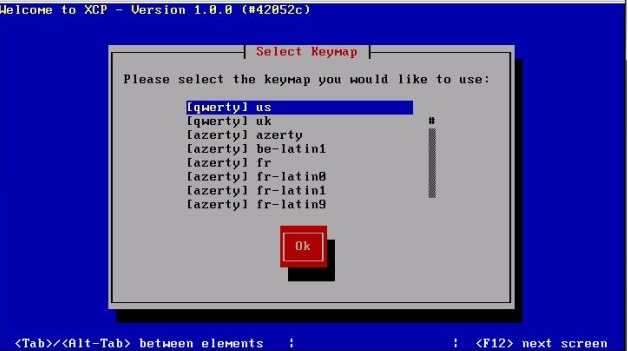
\includegraphics[width=200pt]{images/1.png}
\end{center}
\begin{center}
On choisit le  type de clavier
\end{center}
\begin{center}
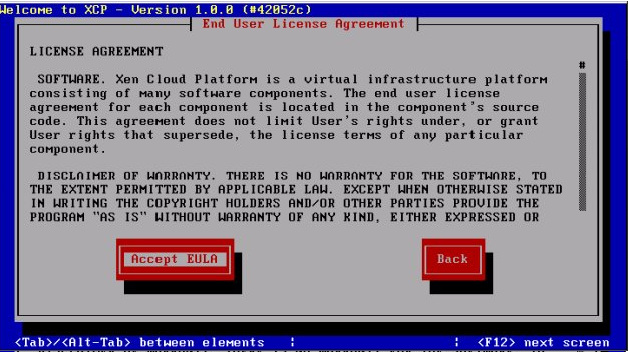
\includegraphics[width=200pt]{images/2.png}
\end{center}
\begin{center}
On accepte la licence
\end{center}
\begin{center}
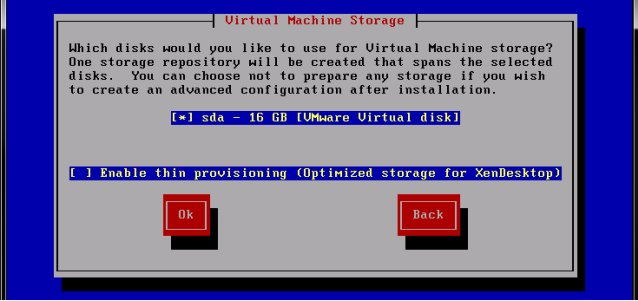
\includegraphics[width=200pt]{images/3.png}
\end{center}
\begin{center}
Choix du disque d'installation
\end{center}
\begin{center}
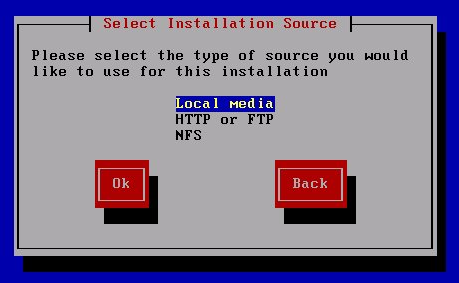
\includegraphics[width=200pt]{images/4.png}
\end{center}
\begin{center}
Choix de la source d'installation
\end{center}
\begin{center}

\includegraphics[width=200pt]{images/5.png}
\end{center}
\begin{center}
Paquets additionnels
\end{center}
\begin{center}
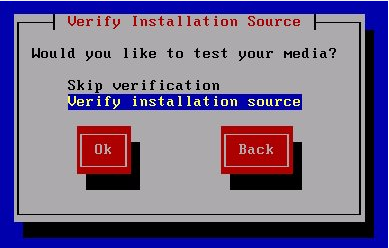
\includegraphics[width=200pt]{images/6.png}
\end{center}
\begin{center}
Vérification de la source d'installation
\end{center}
\begin{center}
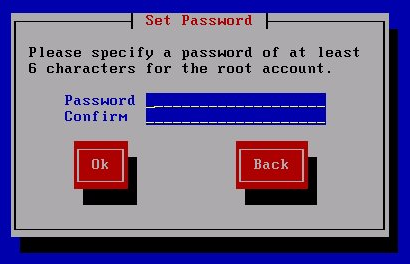
\includegraphics[width=200pt]{images/7.png}
\end{center}
\begin{center}
Choix du password
\end{center}
\begin{center}
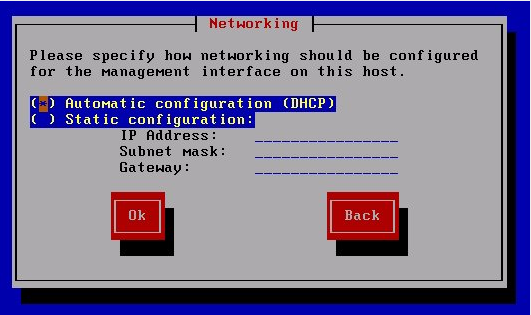
\includegraphics[width=200pt]{images/8.png}
\end{center}
\begin{center}
Configuration du réseau
\end{center}
\begin{center}
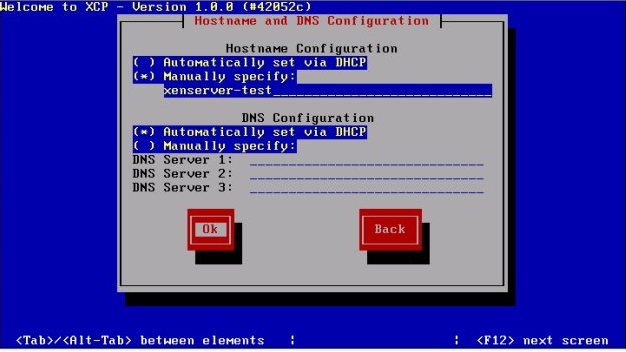
\includegraphics[width=200pt]{images/9.png}
\end{center}
\begin{center}
Configuration du DNS
\end{center}
\begin{center}

\includegraphics[width=200pt]{images/10.png}
\end{center}
\begin{center}
Installation
\end{center}
\begin{center}
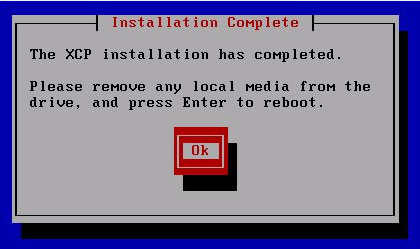
\includegraphics[width=200pt]{images/11.png}
\end{center}
\begin{center}
Installation complète
\end{center}
\begin{center}
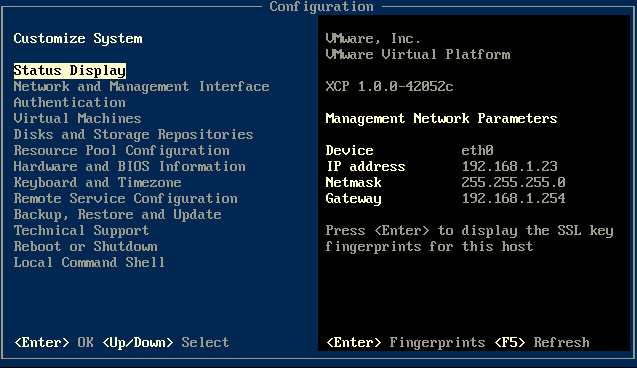
\includegraphics[width=300pt]{images/xcp.png}
\end{center}
\begin{center}
Interface de Xen Cloud Platform
\end{center}
\section{Connexion d'OpenXenManager avec XCP}
Désormais, il est possible de nous connecter avec OpenXenManager sur XCP, il nous suffit de remplir le champ hostname avec l'adresse IP du serveur.
On indique ensuite le port 80 comme port de connexion, et l'on finit par les login et mots de passe.
\begin{center}
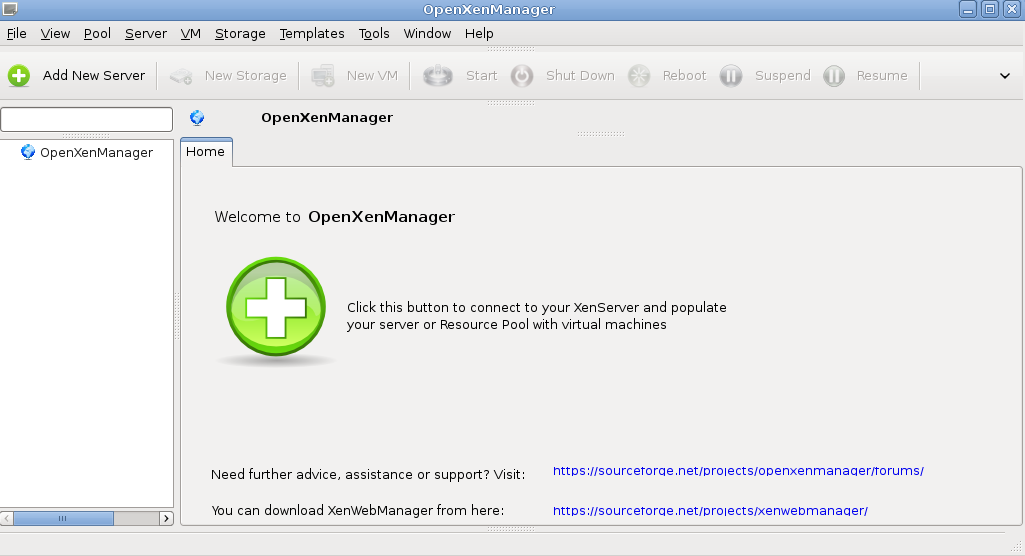
\includegraphics[width=400pt]{images/xenmanager.png}
\end{center}
\begin{center}
Interface graphique
\end{center}
\begin{center}
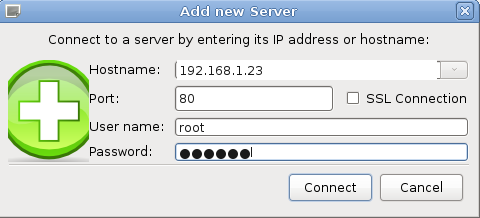
\includegraphics[width=200pt]{images/addserveur.png}
\end{center}
\begin{center}
Ajout du serveur XCP
\end{center}
\begin{center}
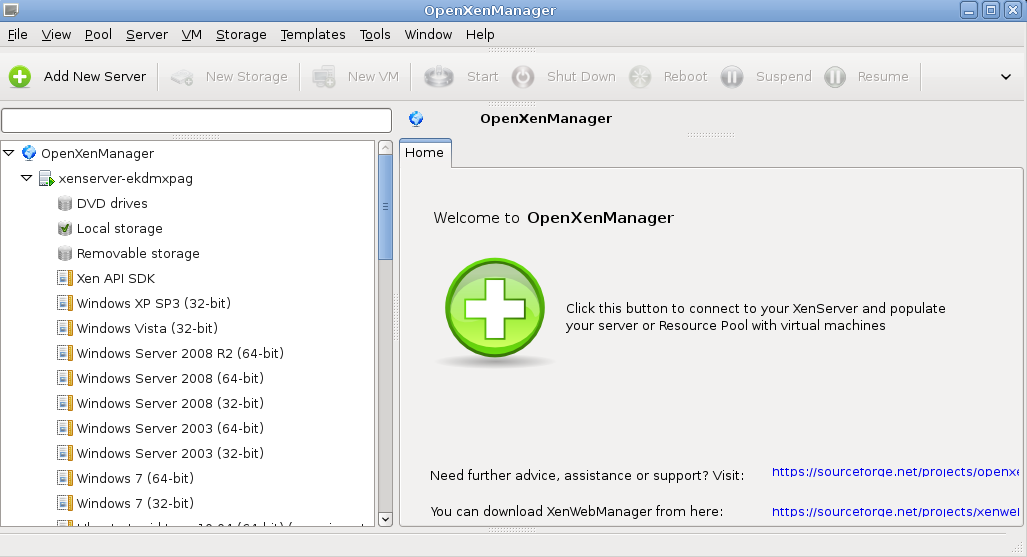
\includegraphics[width=400pt]{images/final.png}
\end{center}
\begin{center}
Vue de toutes les machines virtuelles dans XCP
\end{center}

